\documentclass[10pt]{article}

\usepackage[margin=1in]{geometry}
\usepackage{graphicx}
\usepackage{amsmath}
\usepackage[colorlinks,bookmarks,bookmarksnumbered,allcolors=blue]{hyperref}
\usepackage{booktabs}   % For better tables
\usepackage{enumitem}   % For shorteneted itemize list
\usepackage{titling}    % To adjust title placement

\begin{document}

\title{Wind Farm Layout Optimization Case Studies
\\
\small{IEA Task 37 on System Engineering in Wind Energy}
}
\author{\large Nicholas F. Baker,\  Andrew P. J. Stanley, \ Jared Thomas, \ and Andrew Ning \\
    {\small Brigham Young University, Provo, Utah, USA}\\
\vspace{-1em}\\
\large Katherine Dykes\\
    \small National Renewable Energy Laboratory, Golden, Colorado, USA}
\setlength{\droptitle}{-5em}
\maketitle

\section{Introduction}

    Two major factors that affect wind farm layout optimization are 1) the optimization approach and 2) the wake model. This document defines two case studies designed to study these factors. One may elect to participate in either or both cases.
    \begin{enumerate}
        \item Optimization-Only Case Study: user chooses optimization approach, wake model is fixed and supplied.
        \item Combined Case Study: user is free to choose both optimization approach and wake model.
    \end{enumerate}

    Participants will (1) optimize turbine locations to maximize annual energy production, (2) submit solutions, and (3) provide details on their methodology.  After all submissions are received, for the Combined Case Study participants will be expected to perform a cross comparison of other participant solutions.  Data will be consolidated, processed, and made available to all participants.

\section{Problem Definition}

    \subsubsection*{Objective}

        The objective of each scenario is to maximize annual energy production, which we define simply as the expected value of aerodynamic power.  The wind resource for each case has a wind rose binned into 16 discrete directions, with a constant wind speed.  In other words:
        \begin{equation*}
            AEP = \left(\sum_{i=1}^{16} f_i P_i\right) 8760 \frac{\textrm{hrs}}{\textrm{yr}}
        \end{equation*}
        where $P_i$ is the power produced for wind direction $i$, and $f_i$ is the corresponding wind direction probability.

    \subsubsection*{Design Variables}

        The design variables are the $(x, y)$ locations of each turbine.
        All locations in this document refer to the hub location.
        Every turbine in the farm is identical, and explicitly defined below in \textbf{Parameters}.

    \subsubsection*{Constraints}

        Each wind farm scenario has a fixed circular boundary centered at $(0, 0)$.  All turbine $(x, y)$ locations must remain on or within this boundary.  No turbine can be less than two rotor diameters from any other turbine.

    \subsubsection*{Parameters}

        The wind turbine is the IEA37 3.35 MW onshore reference turbine \cite{NREL335MW} with the following characteristics:
        \begin{center}
            \begin{tabular}{@{}lrl@{}}
            \toprule
                Rotor Diameter & 130 & m \\ 
                Turbine Rating & 3.35 & MW \\ 
                Cut-In Wind Speed & 4 & m/s \\ 
                Rated Wind Speed & 9.8 & m/s \\ 
                Cut-Out Wind Speed & 25 & m/s \\
            \bottomrule
            \end{tabular}
        \end{center}

        \noindent All turbine data is also contained in the enclosed \texttt{iea37-335mw.yaml}. The power curve is defined as:   

        \begin{minipage}{0.53\textwidth}
            \begin{equation*}
                P(V) = 
                \begin{cases} 
                    0 & V < V_{\textit{cut-in}} \\
                    P_{\textit{rated}}\cdot\bigg(\frac{V-V_{\textit{cut-in}}}{V_{\textit{rated}}-V_{\textit{cut-in}}}\bigg)^3 & V_{\textit{cut-in}}\leq V \leq V_{\textit{rated}} \\
                    P_{\textit{rated}} & V_{\textit{rated}} < V < V_{\textit{cut-out}} \\
                    0 & V \geq V_{\textit{cut-out}}
                \end{cases}
            \label{eq:power}
            \end{equation*}
        \end{minipage}\quad
        \begin{minipage}{0.53\textwidth}
            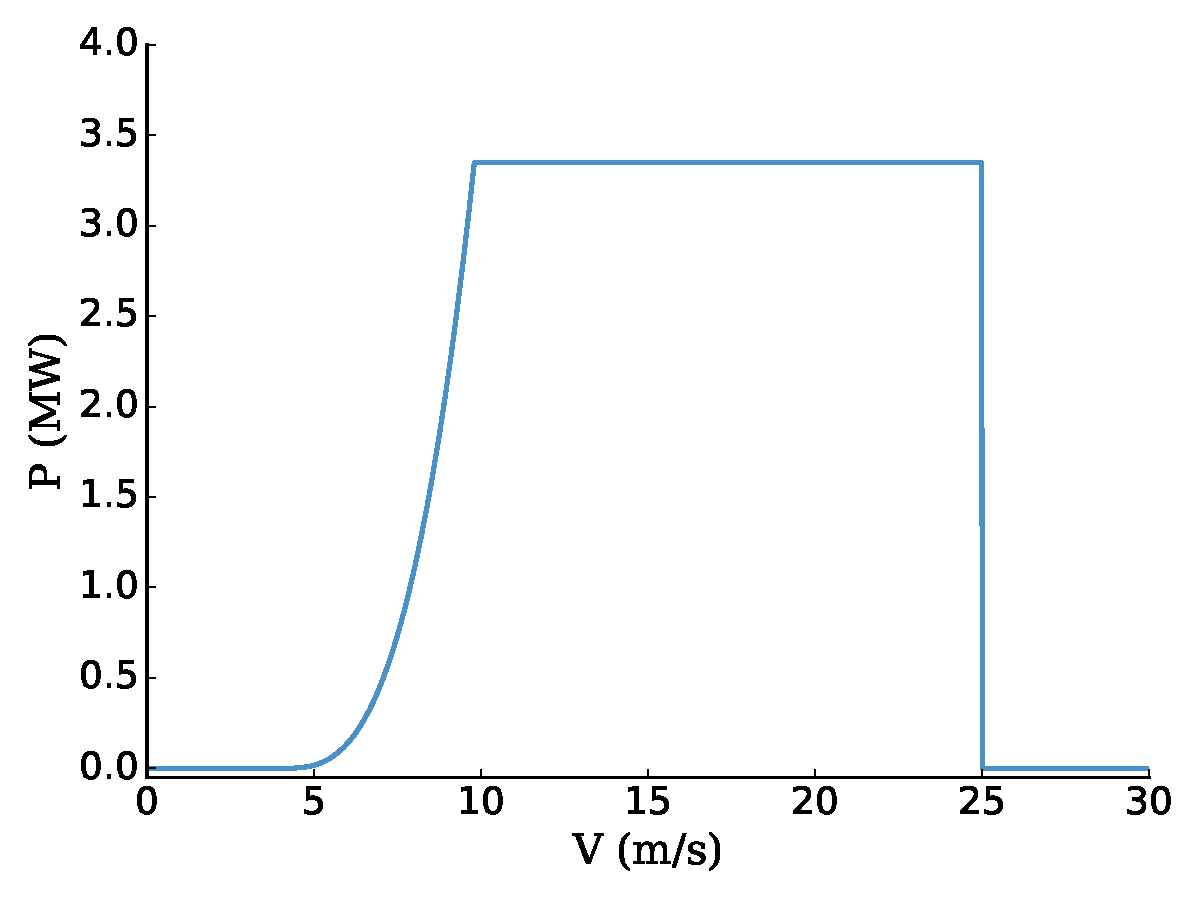
\includegraphics[width=2.6in]{iea37-335mw-pcurve}
        \end{minipage}

        The farm wind speed for all scenarios is constant at 9.8 m/s. North is measured at $0^{\circ}$, and the CW wind rose is defined by 16 discrete bins tabulated in \texttt{iea37-windrose.yaml}, depicted pictorially below:
        \begin{center}
            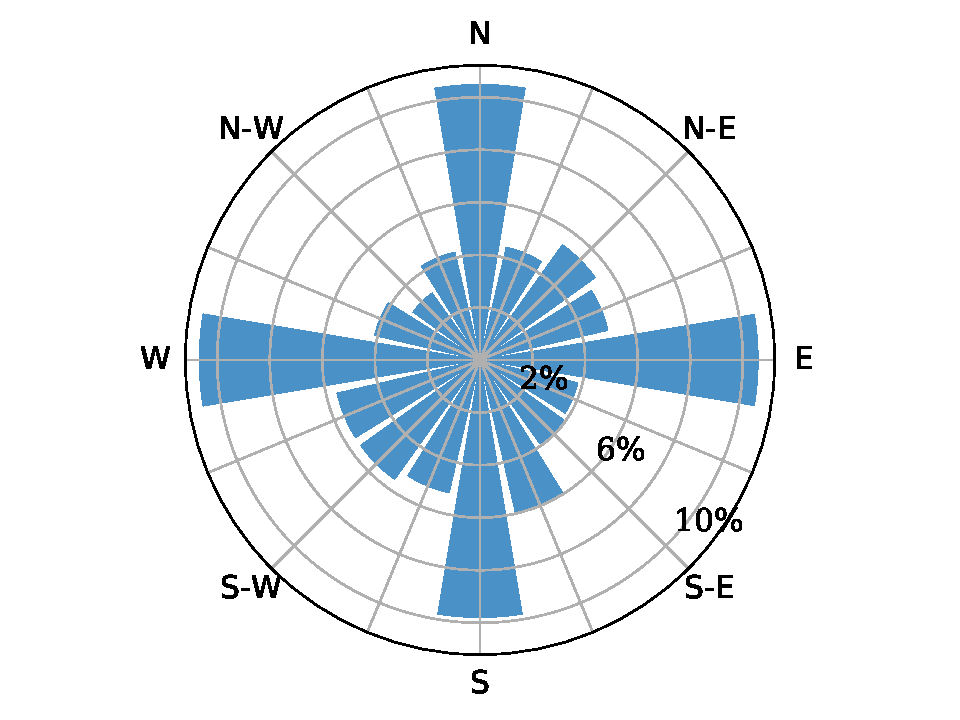
\includegraphics[width=3.5in]{iea37-windrose}
        \end{center}
        
    \subsection{Case Study 1: Optimization Only}

        This problem defines three different wind farm sizes, and corresponding number of turbines, intended to test scalability of your optimization approach.  The three scenarios are:
        \begin{enumerate}
            \item 16 turbines, boundary radius of 1,300 m.
            \item 36 turbines, boundary radius of 2,000 m.
            \item 64 turbines, boundary radius of 3,000 m.
        \end{enumerate}

        For this Case Study the user is only free to choose the optimization approach.
        The wake model is fixed and is a simplified version of Bastankhah's Gaussian wake model \cite{Thomas2018, Bastankhah2014, Bastankhah2016}.
        A Python implementation is supplied for convenience (\texttt{iea37-aepcalc.py}).
        Alterations to this implementation are permitted, as long as the governing physics equations are not altered.
        Participants may use other programming languages, but must use the same physics equations.
        To aid with this, the relevant equations are defined in a separate document (\texttt{iea37-wakemodel.pdf}), and example layouts with corresponding AEP values are provided in \texttt{iea37-ex\#\#.yaml} to verify implementations.
        The example designs are only for verification, and do not need to be used as starting points in your optimization.

    \subsection{Case Study 2: Combined}

        This problem defines one scenario where the user is free to choose both the optimization algorithm and the wake model.
        The single wind farm scenario is nine turbines with a boundary radius of 900 m.
        
        If needed by your wake model choice, the turbulence intensity is 0.075, and the wind shear is a power-law with a shear exponent of 0.15 using the hub height as the reference height.

\section{Reporting and Evaluation}

    Participants will submit:
    \begin{enumerate}
        \item Optimal turbine placement solution for each scenario using the format in the example \texttt{.yaml} files. 
        \item A survey describing your methodology and simulation environment \href{https://goo.gl/forms/2tX3eJ0rlnElmTgR2}{here}.
    \end{enumerate}

    Note that for both Case Studies, your \texttt{.yaml} submissions must report both total farm AEP, and farm AEP for each $\theta$ bin, as in the enclosed \texttt{iea37-ex\#\#.yaml} examples.

    \subsection{Case Study 1: Optimization Only}

        Results will be compared by running the enclosed \texttt{iea37-aepcalc.py}, using the submitted \texttt{.yaml} file from each participant.
        Submissions must adhere to the \texttt{.yaml} format in order to receive a ranking.
        While other implementations may be used in the optimization, all evaluations will be done with the provided \texttt{iea37-aepcalc.py} code, so it is essential that you check that your implementation is consistent.

        Example command-line syntax we will use to evaluate all submitted files is:
        
        \vspace{0.5em}
        \texttt{\$python iea37-aepcalc.py iea37-yourname-opt\#\#.yaml iea37-windrose.yaml iea37-335mw.yaml}
        \vspace{0.5em}
        
        \noindent Where: 
        \begin{itemize}
            \item \texttt{iea37-yourname-opt\#\#.yaml} will be your submitted \texttt{.yaml} with optimal turbine locations.
            \begin{itemize}
                \item ``\texttt{yourname}'' is your personal or organizational name, all lowercase with no spaces or punctuation.
                \item ``\texttt{\#\#}'' is the scenario size, i.e. ``opt16'' would be for the 16-turbine scenario.
            \end{itemize}
            \item \texttt{iea37-windrose.yaml} is the binned wind rose used for both case studies.
            \item \texttt{iea37-335mw.yaml} is the turbine data for the used IEA37 3.35 MW onshore reference turbine.
        \end{itemize}

    \subsection{Case Study 2: Combined}

        Because the wake models differ in this case, determining a ``best'' solution is generally not possible.  Comparisons will be made using two approaches:
        \begin{enumerate}
            \item Every participant will evaluate every other participant's solutions using their own wake model(s).  It is essential that the \texttt{.yaml} format is adhered to so that cross-comparisons are painless. % If the optimizations behave as expected, each participant's wake model will judge their own solution as best, but it is possible a solution is found that other wake models agree is better.
            \item Each solution will be compared using a higher-fidelity simulation, in this case large-eddy simulations (LES) using SOWFA.  This simulation introduces its own modeling assumptions and is an imperfect way to compare, but does provide another piece of information on relative performance between approaches. % It is expected that solutions with minor LES performance differences would lie within the error of the methodology, and thus only major differences will be used in drawing conclusions on relative performance.
        \end{enumerate}

\section{Enclosures}
    Files included with this document, needed for full participation in the Case Studies are:

    \begin{itemize}[noitemsep,topsep=0pt,parsep=0pt,partopsep=0pt]
        \item \texttt{iea37-aepcalc.py} - Python coding of AEP wake model for the Optimization Only Case Study
        \item \texttt{iea37-wakemodel.pdf} - description of AEP algorithm for the Optimization Only Case Study
        \item \texttt{iea37-windrose.yaml} - binned wind frequency for both Case Studies, in \texttt{.yaml} format
        \item \texttt{iea37-335mw.yaml} - data for reference turbine used in both Case Studies, in \texttt{.yaml} format
        \item \texttt{iea37-ex16.yaml} - 16 turbine scenario example layout
        \item \texttt{iea37-ex36.yaml} - 36 turbine scenario example layout
        \item \texttt{iea37-ex64.yaml} - 64 turbine scenario example layout
    \end{itemize}

\bibliographystyle{aiaa}
\bibliography{iea37-wflocs-announcement}

\end{document}